\documentclass[a4paper, titlepage]{article}

\usepackage{graphicx}
\usepackage[colorlinks = true]{hyperref}
\usepackage[thinc]{esdiff}
\usepackage{matlab-prettifier}
\usepackage{listings}
\usepackage{cite}
\usepackage{amsmath,amssymb,amsfonts}
\usepackage{algorithmic}
\usepackage{graphicx}
\usepackage{textcomp}
\usepackage{xcolor}
\usepackage{multicol}
% \usepackage{float}
\def\BibTeX{{\rm B\kern-.05em{\sc i\kern-.025em b}\kern-.08em
T\kern-.1667em\lower.7ex\hbox{E}\kern-.125emX}}
\usepackage{titling}

\lstdefinelanguage{SPICE}{
  morekeywords={R,C,L,V,I},
  sensitive=false,
  morecomment=[l]{*},
  morestring=[b]",
}

\title{
    \begin{center}
        \Huge \textbf{Four-Bit ALU}
    \end{center}
    \vspace{0.5cm}
    \textbf{Final Project} - VLSI (EC2.201)\\
}
\author{
    \textbf{Soham Vaishnav}\\ 
    2022112002\\
    \textit{soham.vaishnav@research.iiit.ac.in}
}

\setcounter{section}{0}

\begin{document}

\maketitle
\tableofcontents

\newpage

\section{About ALU}
\textbf{ALU} stands for \textbf{A}rithmetic and \textbf{L}ogic \textbf{U}nit.
As the name suggests, this particular unit in the processor is dedicated to all the tasks
that require basic mathematical operations and also the tasks that require manipulation of data 
using basic binary logic operations. The ALU therefore becomes an extremely crucial component of 
a CPU. \newline 
The structure of an ALU consists of registers, counters and blocks of combinational logic 
that serves as the basis of all the arithmetic and logic operations. The registers are used to 
store the data which latches on to the inputs of the ALU as and when required, and all the flow
of data within the ALU is controlled by a clock. \newline 
One of the most prominant blocks of an ALU is a \textbf{MUX} or a \textbf{Decoder}. This block of 
combinational logic helps in enabling the ALU to compute only the operation that has been asked for
by the user. It does this by keeping a set of \textbf{select lines} that \textit{choose} what function 
to perform. The choice is realised in the form of an \textbf{enable} to that particular arithmetic or 
logic block of combinational logic. A very crude visualisation of an ALU is given in \hyperlink{ALU}{Fig.1}.

\begin{figure}[htp]
\centering
\hypertarget{ALU}{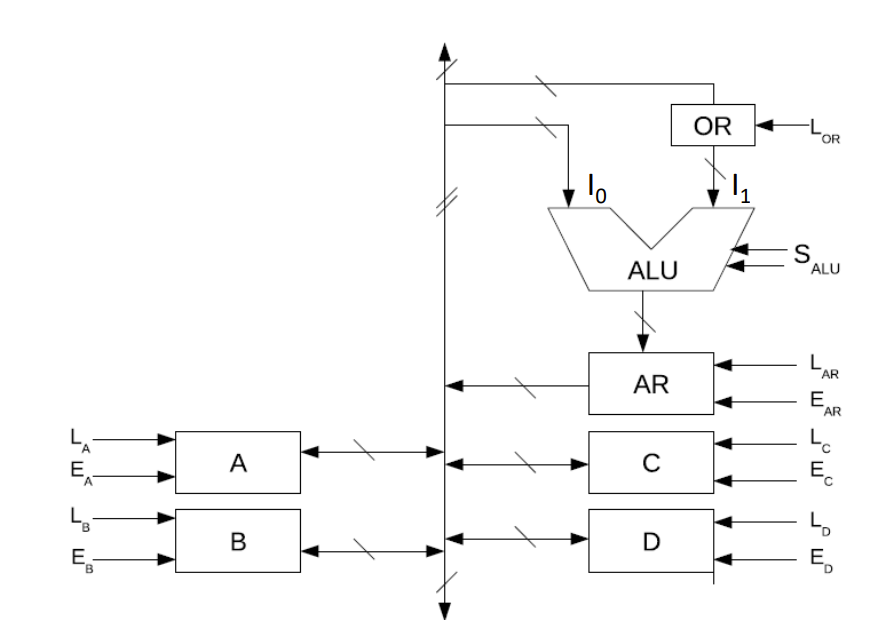
\includegraphics[width=\textwidth]{Image_ALU.png}}
\caption{Basic Design of an ALU}
\label{fig:sysfig}
\end{figure}

\section{Project - Four-bit ALU}
The project aims to impart the knowledge of designing a simple 4-bit ALU that performs operations 
such as Addition, Subtraction, Comparison and ANDing - all applied on two 4-bit numbers. The project
also requires us to perform delay analysis on the operations carried out in order to find 
the maximum or the worst case delay for each of them.\newline 
The tools required to complete the project are - 
\begin{itemize}
    \item \textbf{Verilog} - for logic-level coding 
    \item \textbf{NGSpice} - for coding gate-level netlist
    \item \textbf{MAGIC} - for designing the layout and verify whether the previously designed gate
    netlist complies with the resultant layout.
\end{itemize}

\section{Building the Individual Blocks}
This section deals with the approach taken to build the individual blocks which 
when put together, will result into a 4-bit ALU. The reasoning behind a particular design has also been
discussed alongside. (\textbf{4-bit ALU} block in \textbf{Section}~\ref{sec:Appendix})
\subsection{2x4 Decoder and Enabler}
To select a particular function/operation to be performed on the two 4-bit input 
numbers, as discussed, we need either a MUX or a Decoder. \newline
In this project we make use of a \textbf{2x4 Decoder}. We chose this because we have four operations to
perform - Addition, Subtraction, Comparison and ANDing - and to use a MUX for this seems over-usage of 
combinational logic which renders less efficiency. Also, there is no input in the first place except for 
the select lines and therefore the task can also be completed using a simple Decoder as stated. \newline
The functional aspects of the Decoder used here are as follows - 
(Note that the select lines are named as \textbf{Sel0} and \textbf{Sel1})

\begin{table}[h]
\begin{center} 
\hypertarget{dec_tab}{
\begin{tabular}{|c|c|c|}
    \hline 
    \textbf{Sel0} & \textbf{Sel1} & \textbf{Operation} \\
    \hline
    0 & 0 & Addition \\
    \hline 
    0 & 1 & Subtraction \\
    \hline 
    1 & 0 & Comparison \\
    \hline 
    1 & 1 & ANDing \\
    \hline
\end{tabular}}
\caption{Functional aspects of the Decoder}
\label{tab:t1}
\end{center}
\end{table}
Now based on the table above we design the Decoder with the following design - 
\begin{figure}[htp]
    \centering
    \hypertarget{Dec}{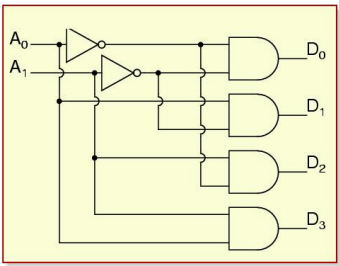
\includegraphics[scale = 0.6]{Image_Decoder.png}}
    \caption{2x4 Decoder}
    \label{fig:fig1}
\end{figure}

Infering from \hyperlink{Dec}{Fig.2}, \textbf{A0} and \textbf{A1} stand for select lines \textbf{Sel0}
and \textbf{Sel1} respectively. Also, logically based on \hyperlink{dec_tab}{Table 1}, \textbf{D0} 
corresponds to \textbf{Addition}, \textbf{D1} to \textbf{Subtraction}, \textbf{D2} to \textbf{Comparison} and 
\textbf{D3} to \textbf{ANDing}. These outputs of the Decoder therefore serve as the \textit{Enables} (\textbf{En}) 
for the functional combinational blocks. Logic can be found in \textbf{Section}~\ref{sec:Appendix}\newline 
\textbf{Note} - We will apply the enables to the output of each operational blocks rather than applying it 
to the inputs to those blocks. The reasons are discussed below-
\begin{itemize}
    \item To reduce the number of gates used which will therefore reduce the area of the layout 
    \item By applying enables to the inputs, we will create an issue for the Comparator, especially when it isn't to 
    be used because then all the \textit{effective} inputs to the comparator will be 0 which will basically signal it to 
    output a logic high at the \textbf{Eql}, thereby indicating that the inputs are equal, which is what we do not want 
    when other some other block is under use
\end{itemize}

\subsection{Operational Blocks}
In this subsection, we will discuss the designing (combinational logic) of the four functional blocks.
\subsubsection{4-bit Adder/Subtractor}
Basic idea here is to make a common block for carrying out addtion and subtraction simply by a \textit{switching}
mechanism which will be driven by the select lines chosen by the user. Reason behind doing this is to primarily
reduce the repetition of blocks because subtraction for radix-2 numbers is basically adding the 2's compliment 
of the subtrahend to the minuend. \newline 
The mechanism for taking a 2's compliment of an n-bit number is 2-step process-
\begin{itemize}
    \item XOR all the bits with 1 which inverts them 
    \item Add 1 to the resultant number
\end{itemize}
One another design principle that we use for designing a basic adder is making use of full-adders. In our case 
since we are adding two 4-bit numbers, we make use of four full-adders with the first full-adder having a carry \textbf{C0}
as an input and the for the remaining full-adders, the carry to those will be the output carry of the immediate previous 
full-adder. Since we are adding two 4-bit numbers, it is very much likely that we get a 5-bit number as an output, where
the $5^{th}$ bit (or the MSB) will be the output carry of the last full-adder. \newline 
Now, we want this same block to work as an adder or as a subtractor based on the select lines that the user chooses. 
Therefore, based on the subtraction steps discussed earlier and using basic digital logic schemes
we note that if we XOR all bits with 1, they get inverted 
and if we XOR them with 0, they remain the same, and if subtraction is to be performed, we put the first carry as 1 (to get
2's complimentof the subtrahend), otherwise 0. Overall, the first carry will be the bit with which we XOR the bits of the
second number. (\textbf{Section}~\ref{sec:Appendix})\newline 
Keeping these design principles in mind we follow the design as shown in \hyperlink{4AS}{Fig.3}. 
Note that in the figure, \textbf{FA} stands for Full-Adder and $A_i$ and $B_i$ are the bits of the 
two numbers. $S_i$ are the bits of the output and $C_i$ are the carries. $C_0$ is the first carry 
which is equal to $M$ - the bit with which we XOR the bits $B_i$.
\begin{figure}[htp]
    \centering
    \hypertarget{4AS}{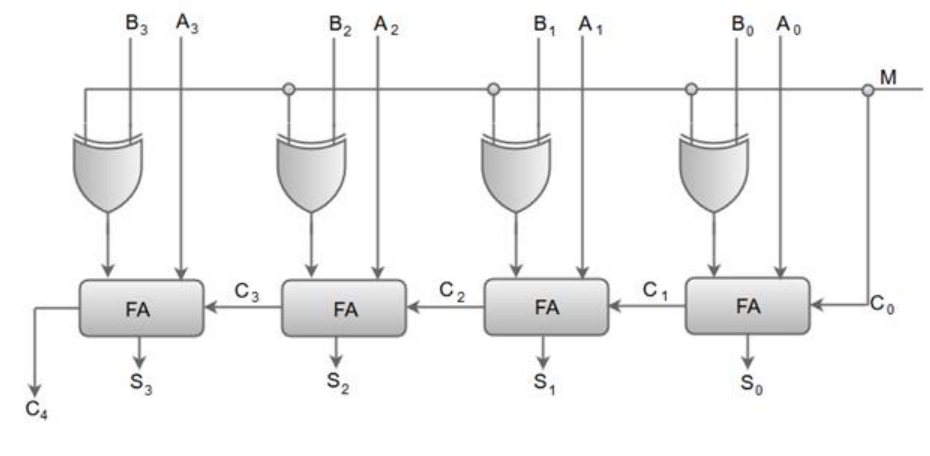
\includegraphics[scale = 0.6]{Image_4-bit_Add-Sub.png}}
    \caption{4-bit Adder/Subtractor}
    \label{fig:fig2}
\end{figure}

\subsubsection{4-bit Comparator}
The 4-bit Comparator does, as the name suggests, comparison between the two input numbers. The outputs to this 
block are therefore \textbf{Eql}, \textbf{Gth} and \textbf{Lth} which stand for \textbf{Equal}, \textbf{Greater-than} and 
\textbf{Less-than} respectively. It is important to note that we compare \textbf{B with respect to A} and not otherwise. 
The logic for comparing A and B for the three conditions stated above is as follows-
\begin{itemize}
    \item \textbf{Eql} - For this purpose we XNOR $A_i$s and $B_i$s because according to the truth table of XNOR 
    it returns a logic high when both the inputs are equal. Now, any two binary numbers are equal if all their bits are same
    , i.e. all the XNORs must return a logic high. And one of the simplest ways to check this is to pass them though a 
    5-input AND gate (5 because the $5^{th}$ input will be enable (\textbf{En})) which will return 1 only when all its 
    inputs are 1.
    \item \textbf{Gth} - The logic used here is based on the fact that we compare the numbers at the first bit where they differ.
    Therefore, it only makes sense to start from the MSB. If MSB of both the numbers are equal then we move to the second bit
    after MSB. But note that while moving to second bit, we must make sure that the first bits are not equal and therefore we
    also take their XNOR into consideration. This applies to all the bits except for the MSB because there is no bit before that.
    And since we are finding whether $A>B$, at every step we AND $A_i$ with $B_i^c$ alongside ANDing with the XNOR of  all $A_{i-1}$
    and $B_{i-1}$ (again MSB are an exception because no previous bits). Finally we take an OR of the outputs of all the ANDs, which
    will return a logic high if there is at least 1 bit where $A>B$
    \item \textbf{Lth} - The logic here is exactly same as the one used for finding \textbf{Gth}. The only difference will be in the 
    inputs given to the AND gates, where instead of $A_i$ and $B_i^c$, we now give $A_i^c$ and $B_i$. The rest remains same
\end{itemize}
Note that as done for \textbf{Eql}, we AND the final outputs of \textbf{Gth} and \textbf{Lth} (after ORing the outputs from 
individual ANDs) with \textbf{En} that will be the output \textbf{D2} of the decoder. \newline 
Interestingly, by applying Enable at the output end helps us eliminate the confusion regarding the numbers being equal that 
would otherwise have persisted had we applied it at the input end. The logic-netlist for the same has been shown in 
\hyperlink{4C}{Fig.4}. Logic can be found in \textbf{Section}~\ref{sec:Appendix}.
\begin{figure}[htp]
    \centering
    \hypertarget{4C}{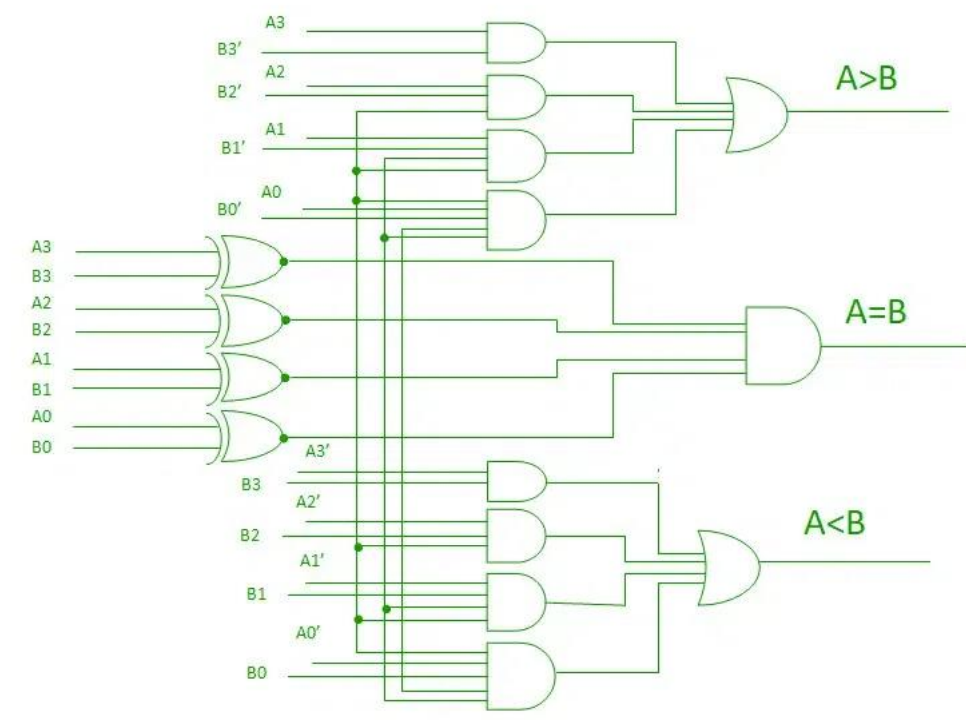
\includegraphics[scale = 0.6]{Image_4-bit_Comparator.png}}
    \caption{4-bit Comparator}
    \label{fig:fig3}
\end{figure}

\subsubsection{4-bit ANDer}
This is the simplest of all blocks in terms of its combinational logic. As the name suggests, we simply have to AND all
the bits $A_i$ with bits $B_i$ and whatever results will be the 4-bit number which will be an ANDed version of the two inputs.
The combinational logic has been demonstrated in \hyperlink{4A}{Fig.5}.
\begin{figure}[htp]
    \centering
    \hypertarget{4A}{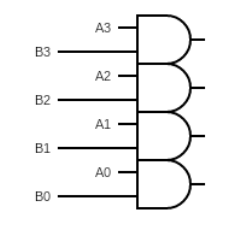
\includegraphics[scale = 1]{Image_4-bit_ANDer.png}}
    \caption{4-bit ANDer}
    \label{fig:fig4}
\end{figure}
Note that the outputs from each of these blocks will be further ANDed with \textbf{En} to comply with 
our original idea of ANDing the enables to the outputs. Therefore, keeping this in mind, it would rather be better 
to use 3-input AND gates which will reduce the transistor count by 10 in total. Logic in \textbf{Section}~\ref{sec:Appendix}.
\\\\
With this we end this section where all the designs have been discussed.

\section{Tools/Platforms used for Building}
Here, we explore the tools used to realise the logic for the combinational circuits discussed in the previous section.
Three most fundamental tools have been used to build this each of which is discussed elaborately.
\subsection{Verilog}
Verilog helps in realising the logic-level coding which is basically the first step in ensuring that the logic we came up with 
was correct and does indeed work the way it was intended. To make coding simpler, we make use of \textbf{modules} of each block 
which made the code look more decipherable. The code and has been shown below-
\begin{multicols}{2}
\setlength{\columnseprule}{0.4pt}
\begin{lstlisting}[language = Verilog]
module two_four_Decoder
(
    input [1:0] Sel,
    output [3:0] Y
);
and (Y[0],~Sel[1],~Sel[0]);
and (Y[1],~Sel[1],Sel[0]);
and (Y[2],Sel[1],~Sel[0]);
and (Y[3],Sel[1],Sel[0]);
endmodule


module full_adder
(
    input A,B,C,
    output [1:0] Y
);
wire w1,w2,c;
and (c,A,B);
xor (w1,A,B);

xor (Y[0],w1,C);

and (w2,C,w1);
or (Y[1],c,w2);
endmodule;

module four_bit_Adder_Subtr
(
    input En,
    input C0,
    input [3:0] A,B,
    output [4:0] Y
);
wire [3:0] b;
xor (b[0],C0,B[0]);
xor (b[1],C0,B[1]);
xor (b[2],C0,B[2]);
xor (b[3],C0,B[3]);

wire [1:0] y1,y2,y3,y4;
full_adder f1(A[0],b[0],
C0,y1);
and (Y[0],En,y1[0]);
full_adder f2(A[1],b[1],
y1[1],y2);
and (Y[1],En,y2[0]);
full_adder f3(A[2],b[2],
y2[1],y3);
and (Y[2],En,y3[0]);
full_adder f4(A[3],b[3],
y3[1],y4);
and (Y[3],En,y4[0]);
and (Y[4],En,y4[1]);
endmodule

module four_bit_Comp
(
    input En,
    input [3:0] A,B,
    output Eq,Gt,Lt
);
wire w1,w2,w3,w4;
xnor (w1,A[0],B[0]);
xnor (w2,A[1],B[1]);
xnor (w3,A[2],B[2]);
xnor (w4,A[3],B[3]);
and (Eq,En,w1,w2,w3,
w4);

wire w5,w6,w7,w8,w13;
and (w5,A[3],~B[3]);
and (w6,w4,A[2],~B[2]);
and (w7,w3,w4,A[1],~B[1]);
and (w8,w2,w3,w4,A[0],
~B[0]);
or (w13,w5,w6,w7,w8);
and (Gt,En,w13);

wire w9,w10,w11,w12,
w14;
and (w9,~A[3],B[3]);
and (w10,w4,~A[2],B[2]);
and (w11,w3,w4,~A[1],B[1]);
and (w12,w2,w3,w4,~A[0],
B[0]);
or (w14,w9,w10,w11,w12);
and (Lt,En,w14);
endmodule

module four_bit_ANDer
(
    input En,
    input [3:0]A,B,
    output [3:0] Y
);
and (Y[0],En,A[0],B[0]);
and (Y[1],En,A[1],B[1]);
and (Y[2],En,A[2],B[2]);
and (Y[3],En,A[3],B[3]);
endmodule

module four_bit_ALU
(   
    input [3:0] A,B,
    input [1:0] Sel,
    output [4:0] Y_addSub,
    output [3:0] Y_and,
    output Eq,Gt,Lt
);
wire [3:0] y;

two_four_Decoder D(Sel,y);

four_bit_Adder_Subtr 
f1(!Sel[1],Sel[0],
A,B,Y_addSub);
four_bit_Comp 
f3(y[2],A,B,Eq,Gt,Lt);
four_bit_ANDer 
f4(y[3],A,B,Y_and);
endmodule
\end{lstlisting}
\end{multicols}

\subsection{Ngspice}
Ngspice is a language used to construct the gate-(or transistor)level netlist based on the boolean logic developed in
Verilog. The approach taken here is the one where we declare \textbf{subckts} for individual gates and thereafter blocks.
The main ALU code in Ngspice is shown below-
\begin{multicols}{2}
\setlength{\columnseprule}{0.4pt}
\begin{lstlisting}[language = SPICE]
    .title 4 Bit ALU
    .include TSMC_180nm.txt
    .global gnd
    
    VinSelD0 SelD_0 0 dc 0
    VinSelD1 SelD_1 0 dc 0
    
    VDD vdd 0 1.8
    
    X1 SelD_0 SelD_1 
    y1 y2 y3 y4 vdd 0 
    2_4_Decoder

    X5 y_as 
    A3 A2 A1 A0 B3 B2 B1 B0 
    C_over S3 S2 S1 S0 vdd 0 
    4_bit_Adder_Sub
    
    X6 y3 
    A3 A2 A1 A0 B3 B2 B1 B0 
    Eql Gth Lth vdd 0 
    4_bit_Comparator
    
    X7 y4 
    A3 A2 A1 A0 B3 B2 B1 B0 
    C3 C2 C1 C0 vdd 0 
    4_bit_ANDer
    
    .end
\end{lstlisting}
\end{multicols}
For convenience, the \textbf{subckts} that have to be \textbf{.include}-ed haven't been shown in the above code.

\subsection{MAGIC Layout}
We now reach the final step of creating the 4-bit ALU, i.e. creating the layout using MAGIC. Here, we create the
transistor-level layout using CMOS technology. \textbf{Note} that throughout the project we are using the TSMC 180nm
technology. Therefore, the minimum permitted channel length in this case would be $0.18\mu$m. In MAGIC as well we 
make use of \textbf{subcells} which are blocks of layouts that can be used to make a major layout.
The following set of images shows the layouts of
the major combinational blocks of the 4-bit ALU - \hyperlink{4DM}{Decoder}, \hyperlink{4ASM}{4-bit Add/Sub}, 
\hyperlink{4CM}{4-bit Comparator}, \hyperlink{4AM}{4-bit ANDer} and finally the \hyperlink{4ALUM}{4-bit ALU}.
\begin{figure}[htp]
    \centering
    \hypertarget{4DM}{\rotatebox{90}{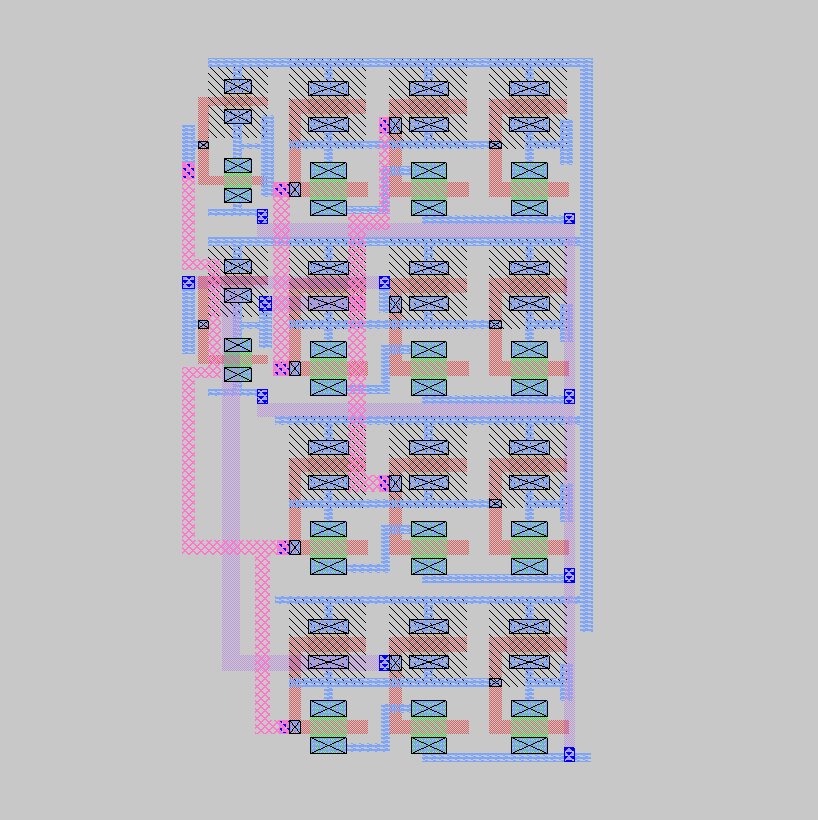
\includegraphics[scale = 0.4]{Image_Decoder_mag.png}}}
    \caption{Decoder Layout using MAGIC}
    \label{fig:fig5}
\end{figure}
\begin{figure}[htp]
    \centering
    \hypertarget{4ASM}{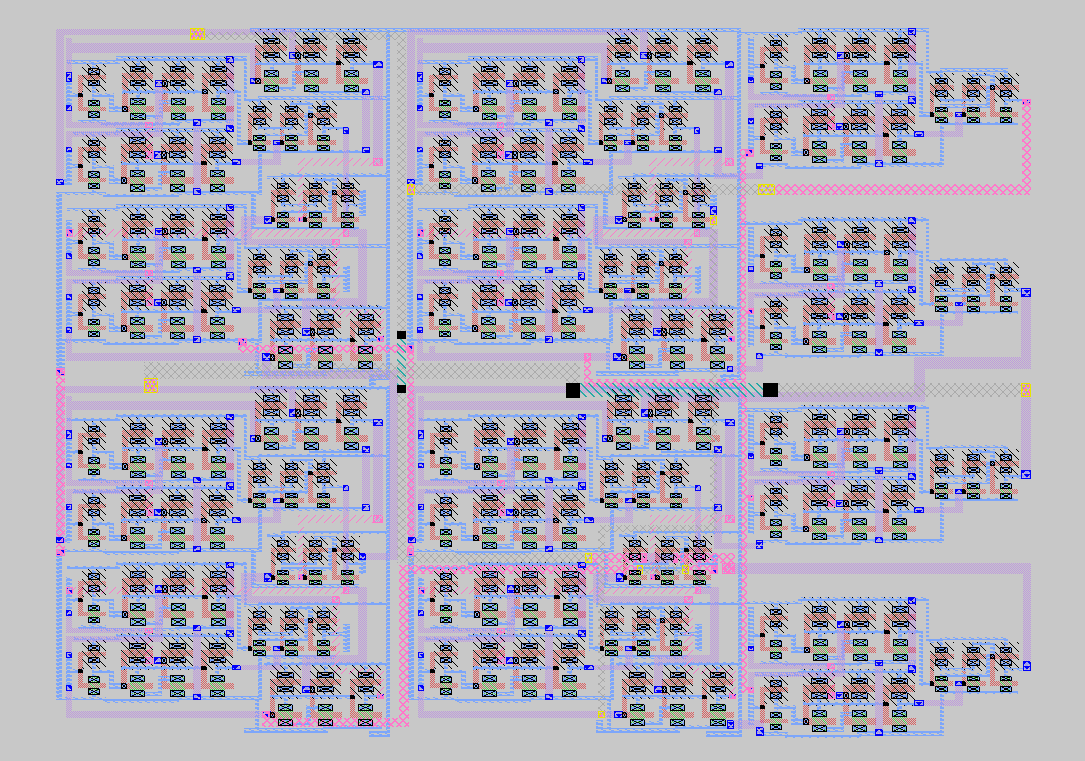
\includegraphics[scale = 0.5]{Image_4-bit_AS_mag.png}}
    \caption{4-bit Adder/Subtractor Layout using MAGIC}
    \label{fig:fig6}
\end{figure}
\begin{figure}[htp]
    \centering
    \hypertarget{4CM}{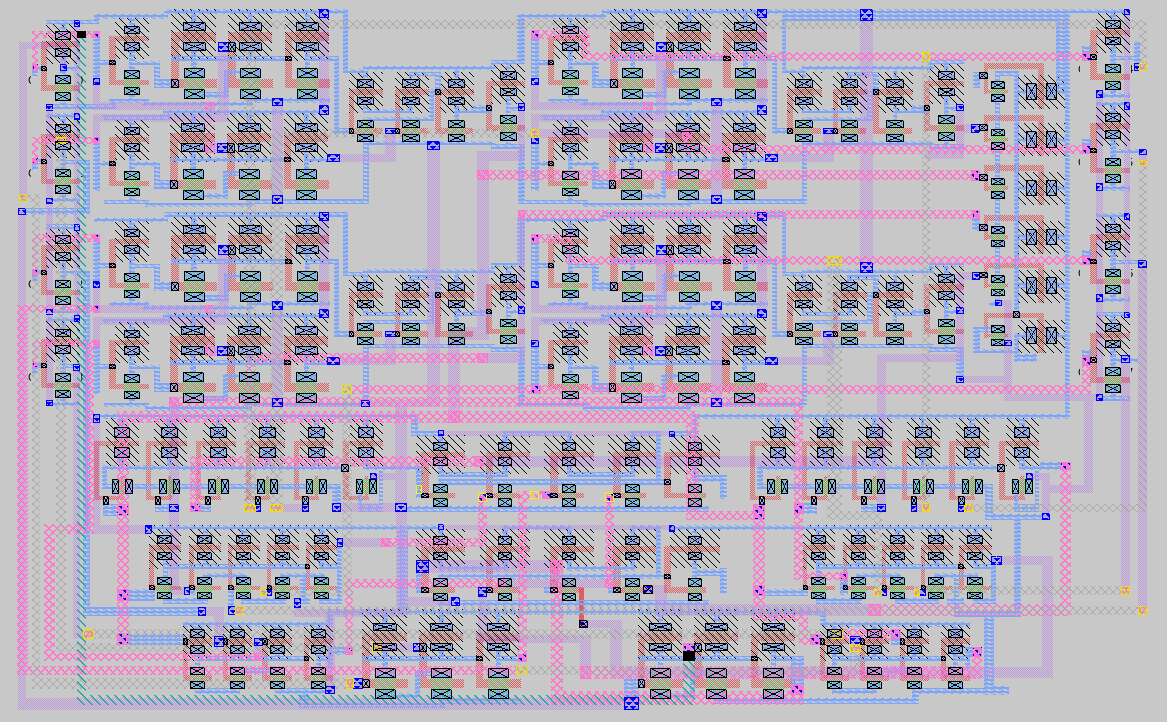
\includegraphics[width = \textwidth, scale = 0.7]{Image_4-bit_Comp_mag.png}}
    \caption{4-bit Comparator Layout using MAGIC}
    \label{fig:fig7}
\end{figure}
\begin{figure}[htp]
    \centering
    \hypertarget{4AM}{\rotatebox{90}{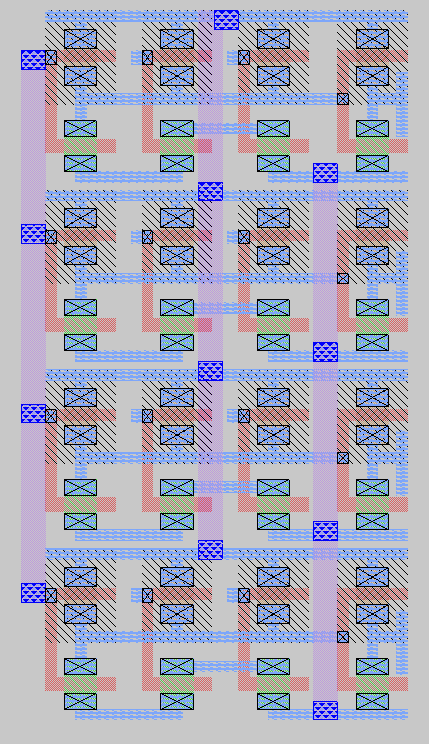
\includegraphics[scale = 0.8]{Image_4-bit_ANDer_mag.png}}}
    \caption{4-bit ANDer Layout using MAGIC}
    \label{fig:fig8}
\end{figure}
\begin{figure}[htp]
    \centering
    \hypertarget{4ALUM}{\rotatebox{270}{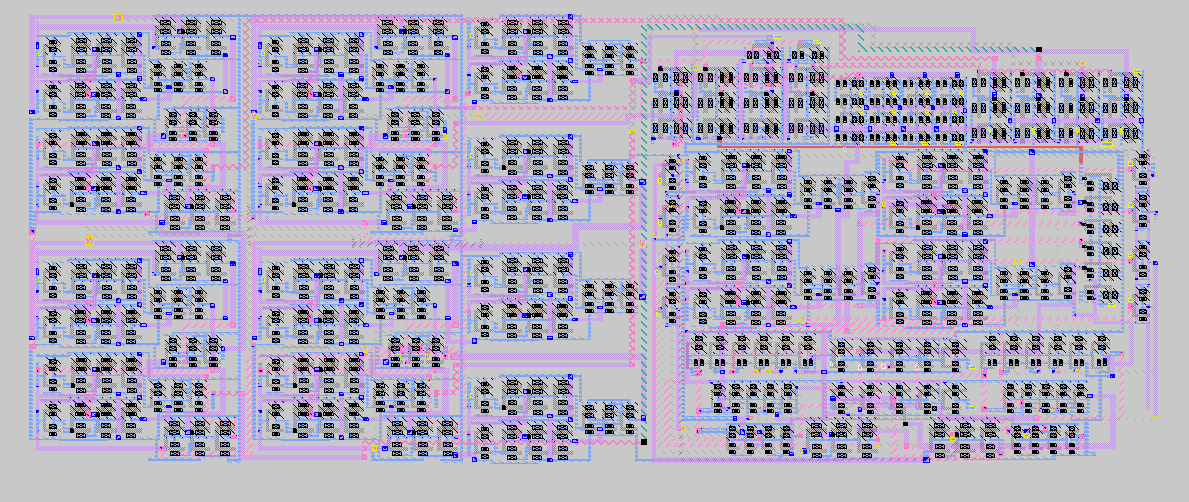
\includegraphics[scale = 0.95]{Image_4-bit_ALU_mag.png}}}
    \caption{4-bit ANDer Layout using MAGIC}
    \label{fig:fig9}
\end{figure}\newline
The main part in MAGIC comes after the layout is made - when we need to convert it back to SPICE in order to check its 
compliance with the gate-netlist that it was originally built from. 

\section{Results and Inference}
Now that all the components are built using all the tools, what's left is verification of the plots, i.e whether 
the blocks are working as intended. For the same, I have posted all the plots obtained after using each of the three 
tools. It is sufficient to paste the plots for the working of the entire ALU which indirectly verifies the working 
of the individual blocks.
\subsection{Verilog}
The plots for different sets of inputs has been shown using verilog as follows:
\begin{figure}[htp]
    \centering
    \hypertarget{GTK1}{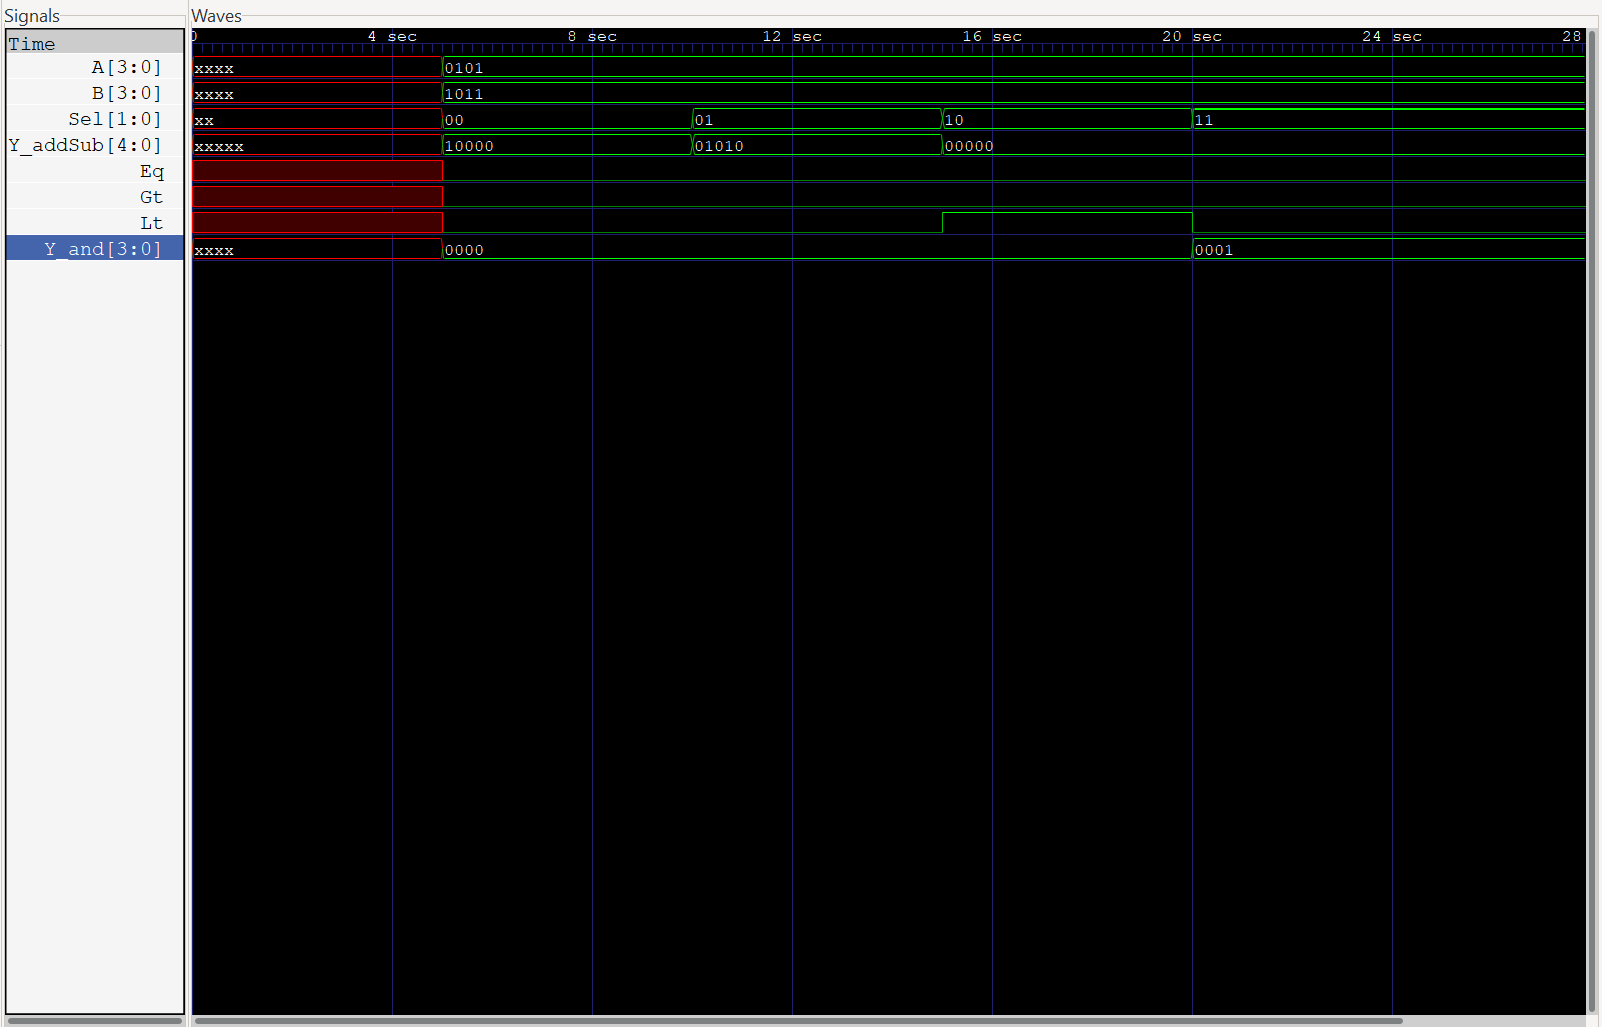
\includegraphics[scale = 0.3]{ALU_Outputs_1_sample.png}}
    \caption{GTK Plot for A=0101 and B=1011}
    \label{fig:fig10}
\end{figure}
\begin{figure}[htp]
    \centering
    \hypertarget{GTK12}{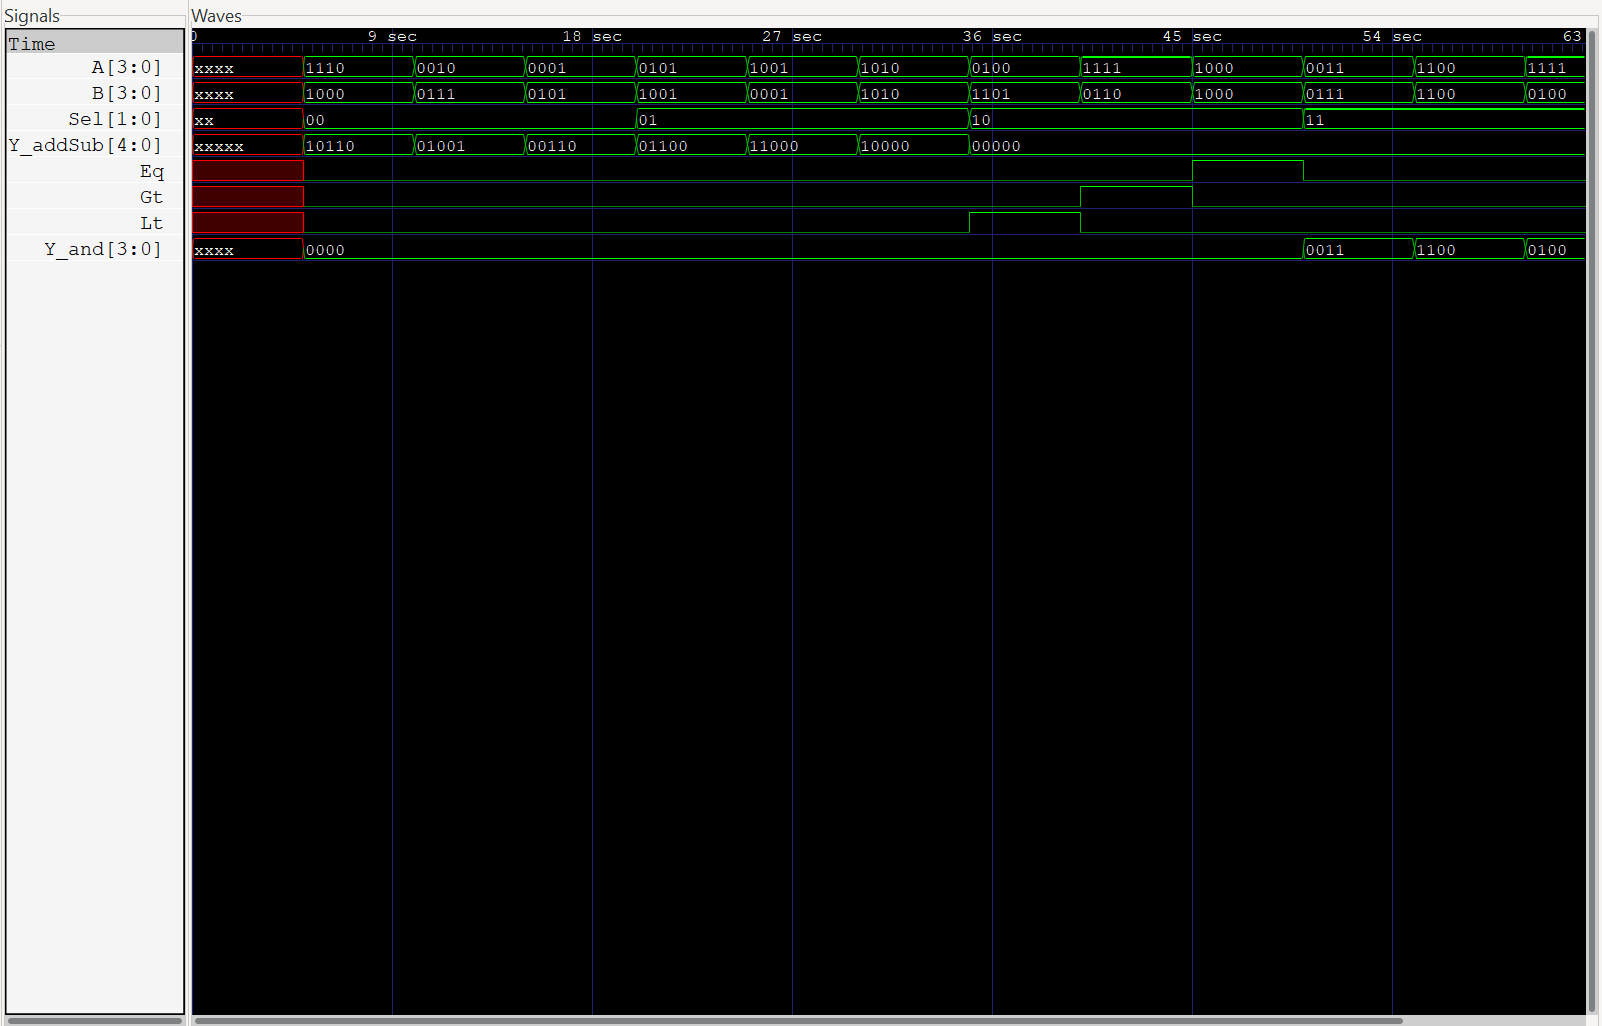
\includegraphics[scale = 0.3]{ALU_Outputs_12_samples.png}}
    \caption{GTK Plot for combinations of different values of A and B}
    \label{fig:fig11}
\end{figure}
\begin{figure}[htp]
    \centering
    \hypertarget{VeriOut12}{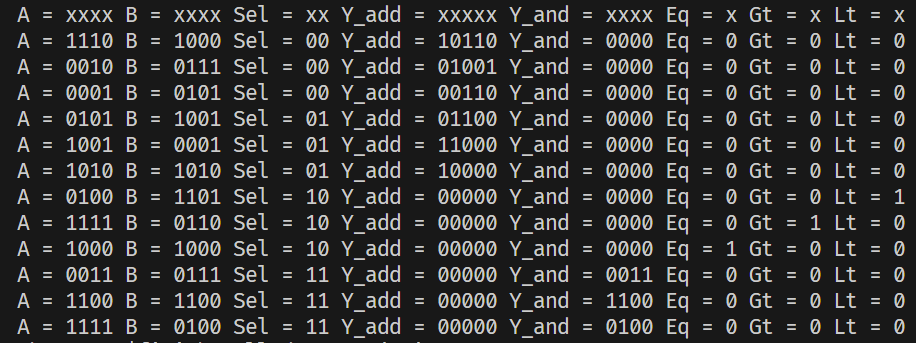
\includegraphics[scale = 0.5]{Output_result_12_samples.png}}
    \caption{Terminal Output for combinations of different values of A and B}
    \label{fig:fig12}
\end{figure}

\subsection{Ngspice}
Here we plot the output waveforms for same (A=0101 and B=1011) input that we had used for Verilog. The plots we therefore get 
are as follows:
\begin{figure}[htp]
    \centering
    \hypertarget{NGA}{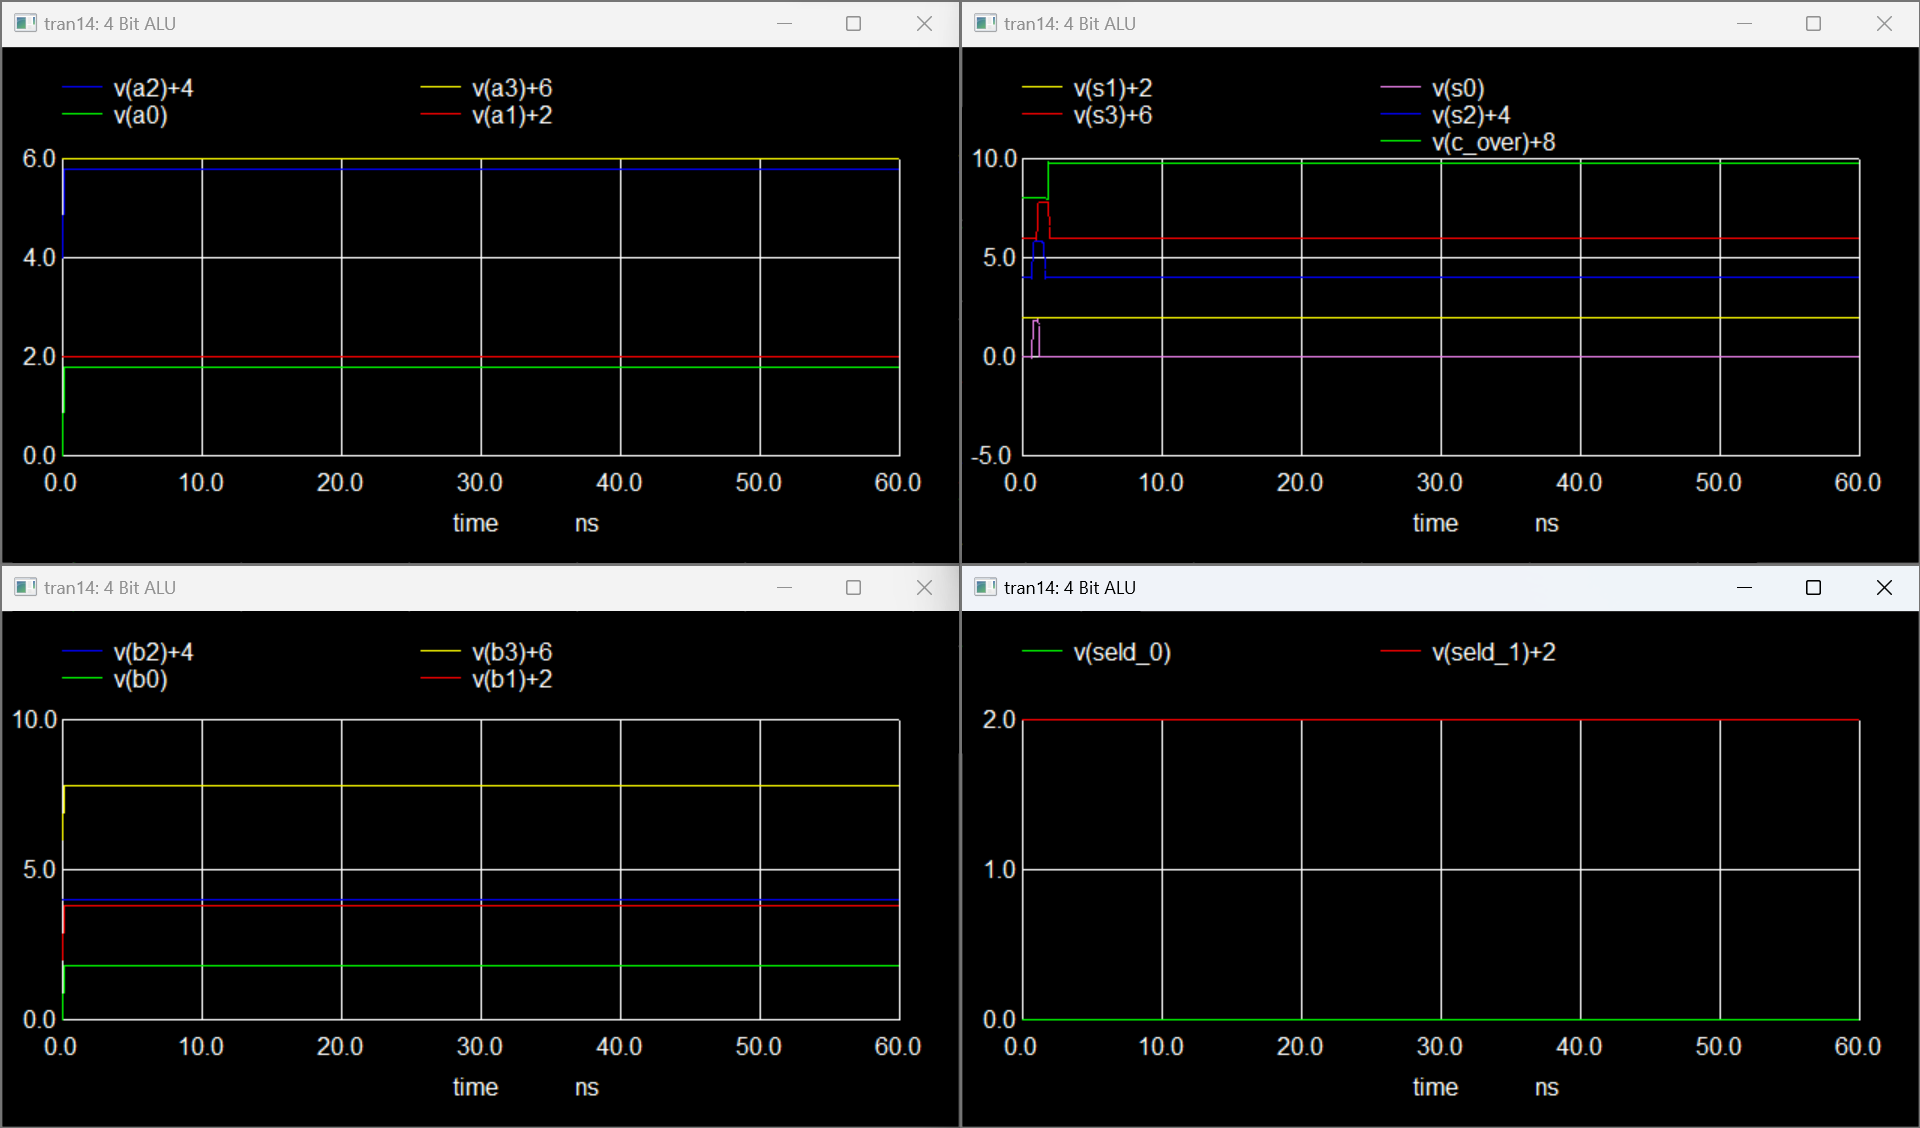
\includegraphics[scale = 0.3]{Adder-Subtractor_output (00-select).png}}
    \caption{Addition}
    \label{fig:fig13}
\end{figure}
\begin{figure}[htp!]
    \centering
    \hypertarget{NGS}{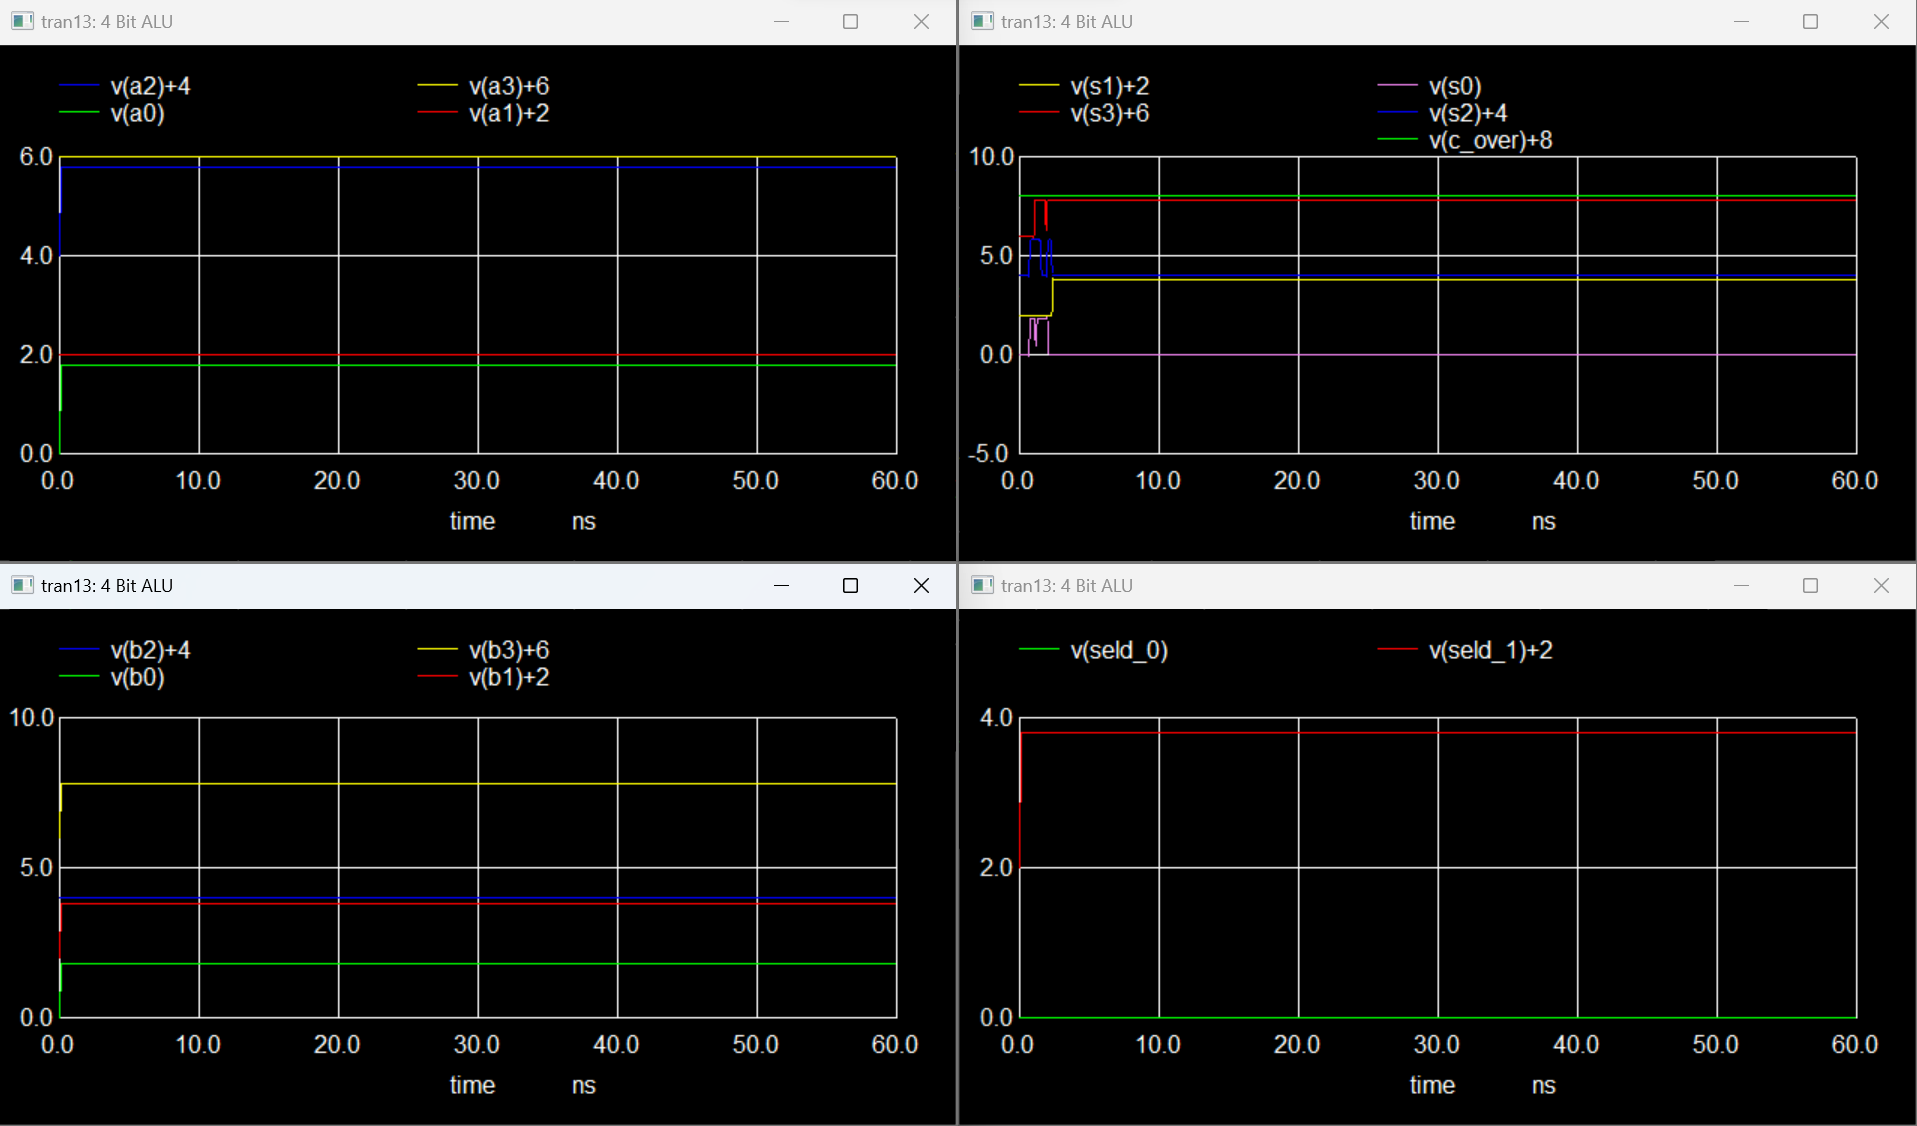
\includegraphics[scale = 0.3]{Adder-Subtractor_output (01-select).png}}
    \caption{Subtraction}
    \label{fig:fig14}
\end{figure}
\begin{figure}[htp!]
    \centering
    \hypertarget{NGC}{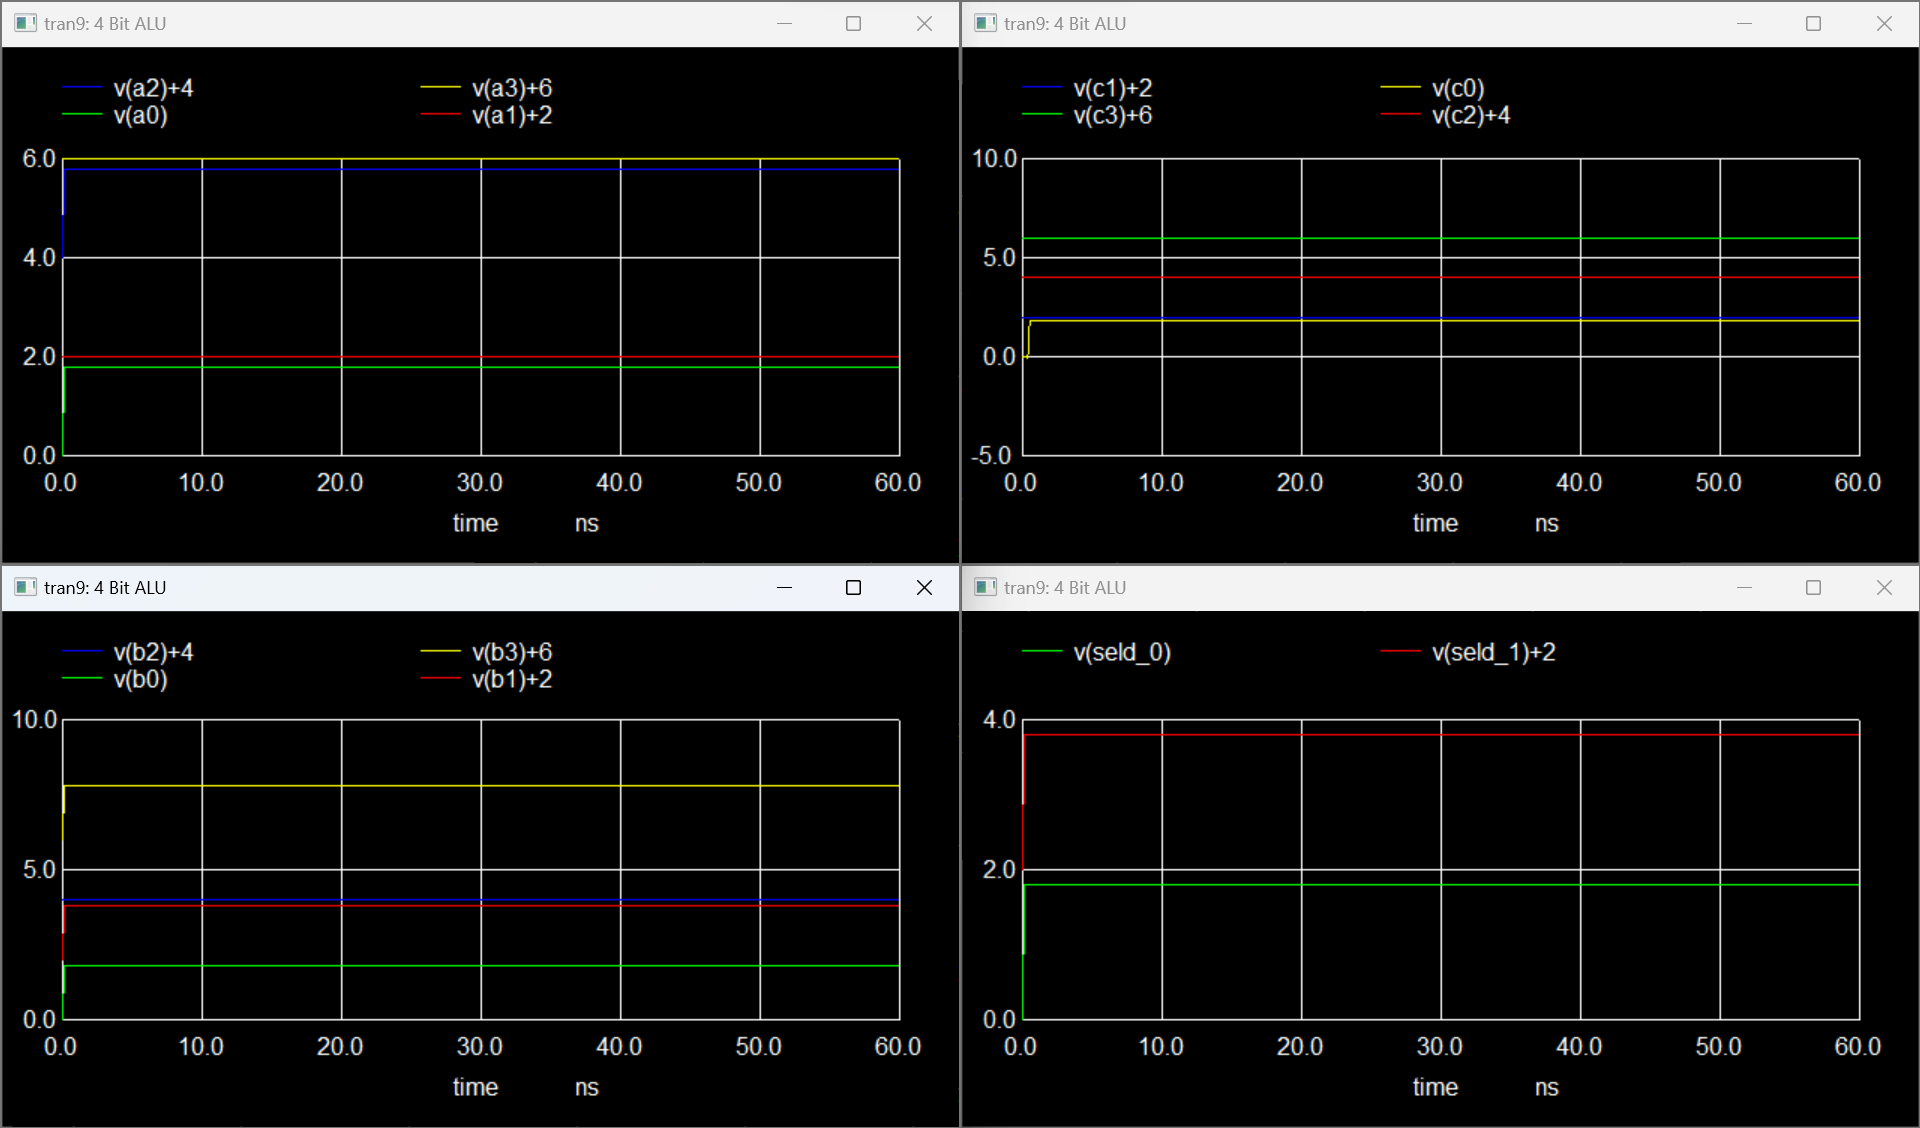
\includegraphics[scale = 0.3]{Comparator_output.png}}
    \caption{Comparator}
    \label{fig:fig15}
\end{figure}
\begin{figure}[htp!]
    \centering
    \hypertarget{NGA}{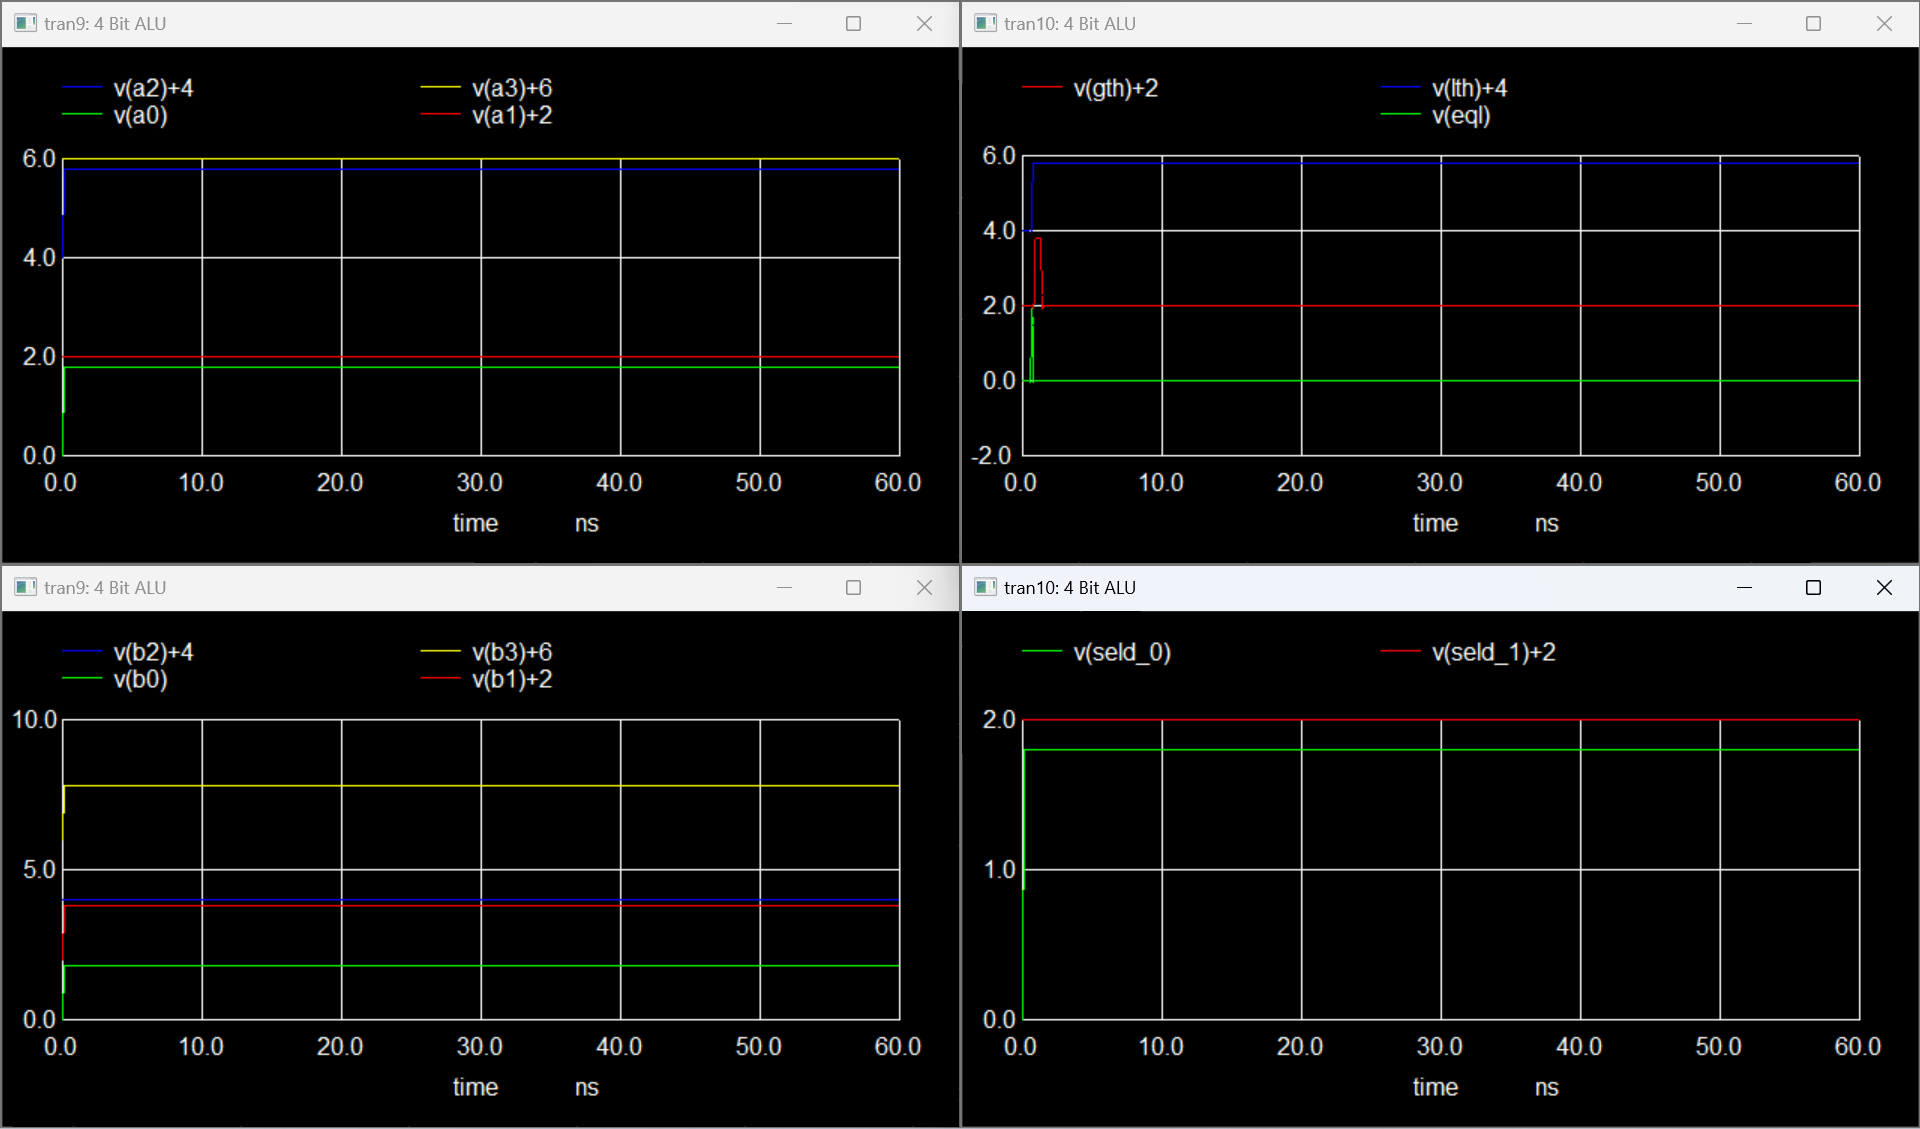
\includegraphics[scale = 0.3]{ANDer_output.png}}
    \caption{ANDing}
    \label{fig:fig16}
\end{figure}

\subsection{MAGIC Layout}
In MAGIC, once the layout is done, as mentioned earlier, we convert it abck to SPICE in order to check whether the layout 
that was made referring to the netlist did turn out the way we wanted it to, i.e. it is giving desired output for desired 
set of inputs. \newline 
Furthermore, the outputs obtained on the SPICE files made from MAGIC layout show us the "real" picture as to how will the 
output look once the layout is fabricated and made into an IC. The delays in this case are the closest to the ones you 
can get in real life.\newline 
Elaborating on the previous point, if closely observed, the layout outputs will have a lightly larger delay in their outputs
as compared to those in the NGSpice plots due to the use of actual parametrised transistors used in layout.
The plots thus obtained are as follows: (Note: A=0101 and B=1011)
\begin{figure}[htp!]
    \centering
    \hypertarget{MA}{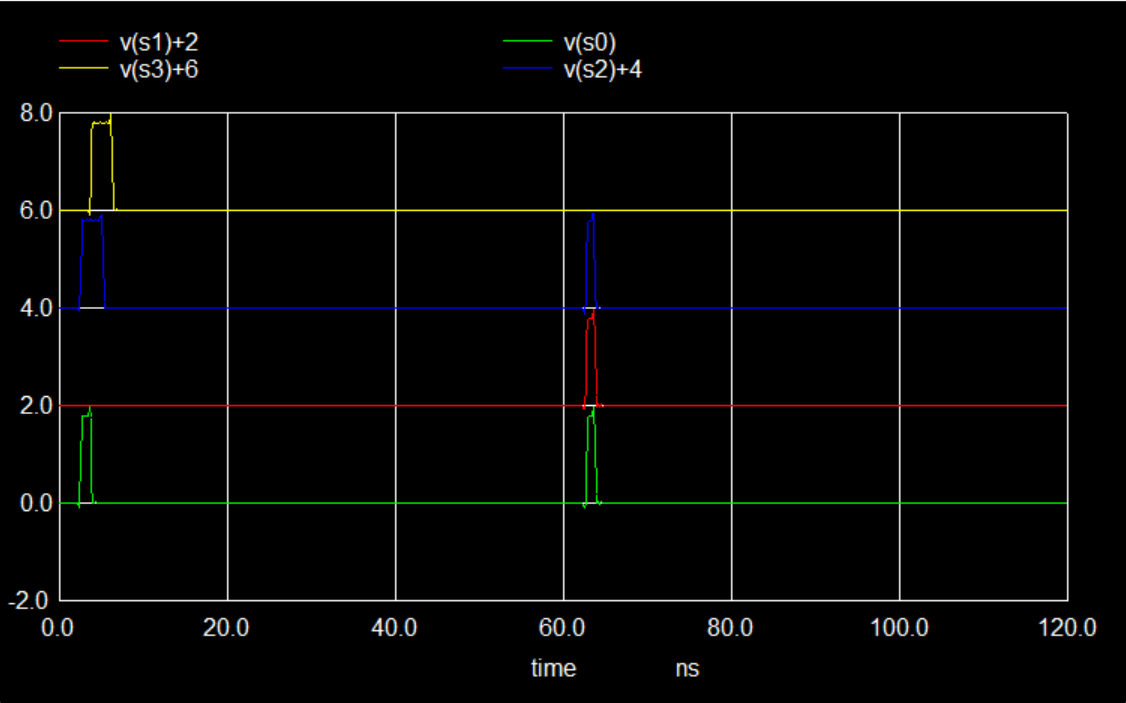
\includegraphics[scale = 0.5]{4_bit_AS_00.png}}
    \caption{Addition}
    \label{fig:fig17}
\end{figure}
\begin{figure}[htp!]
    \centering
    \hypertarget{MS}{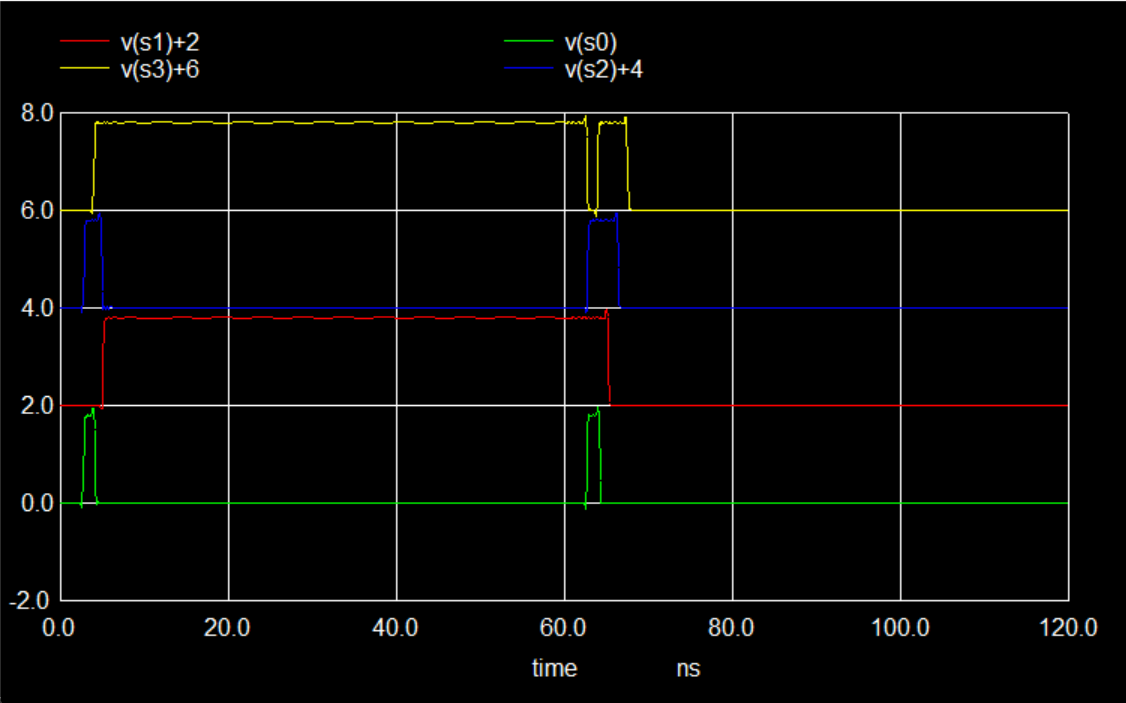
\includegraphics[scale = 0.5]{4_bit_AS_01.png}}
    \caption{Subtraction}
    \label{fig:fig18}
\end{figure}
\begin{figure}[htp!]
    \centering
    \hypertarget{MC1}{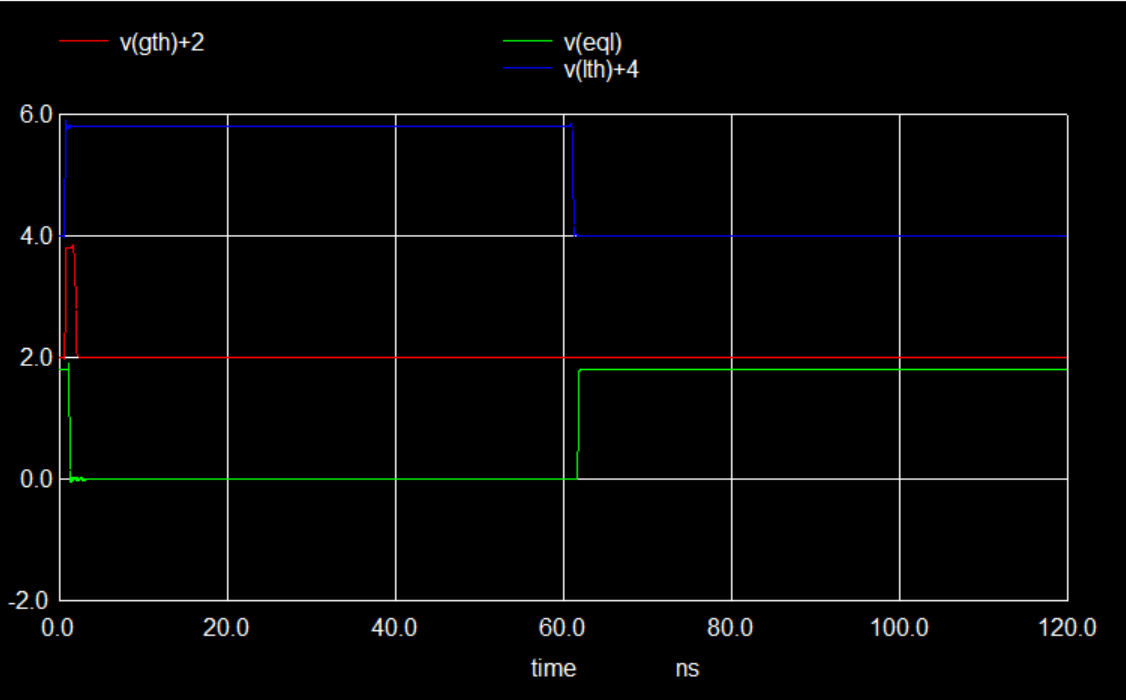
\includegraphics[scale = 0.5]{4_bit_C_10.png}}
    \caption{Comparison}
    \label{fig:fig19}
\end{figure}
\begin{figure}[htp!]
    \centering
    \hypertarget{MC2}{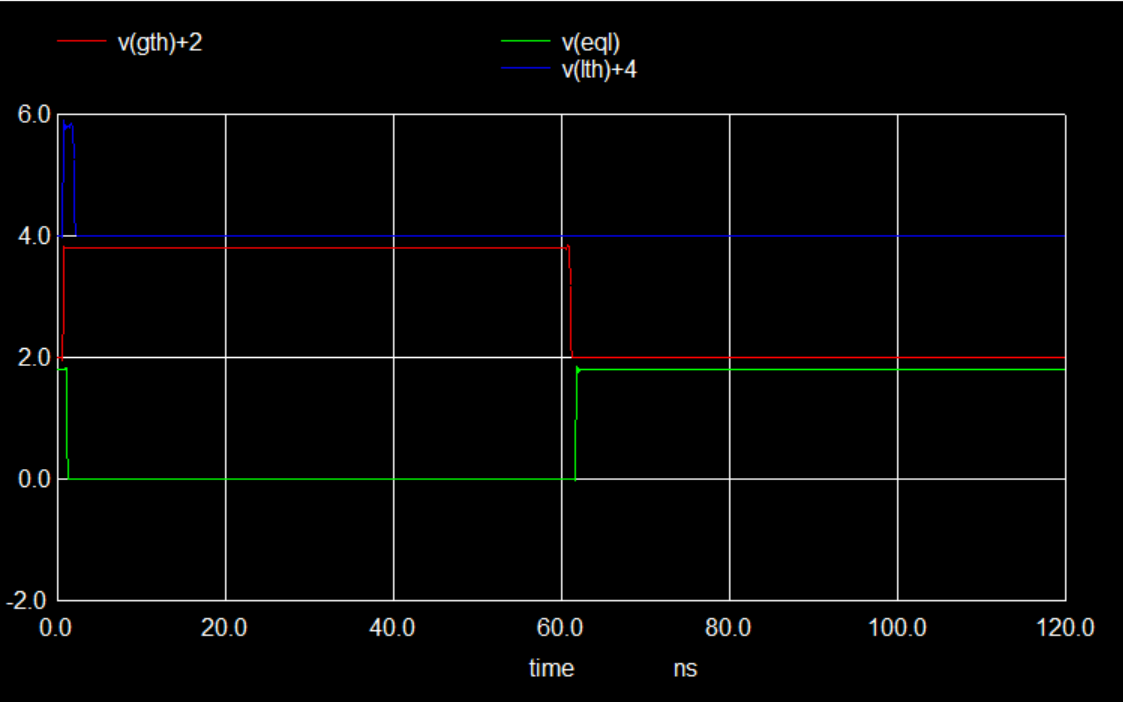
\includegraphics[scale = 0.5]{4_bit_C_10_diffIn.png}}
    \caption{Comparison with inputs A=0101 and B=0011}
    \label{fig:fig20}
\end{figure}
\begin{figure}[htp!]
    \centering
    \hypertarget{MAnd}{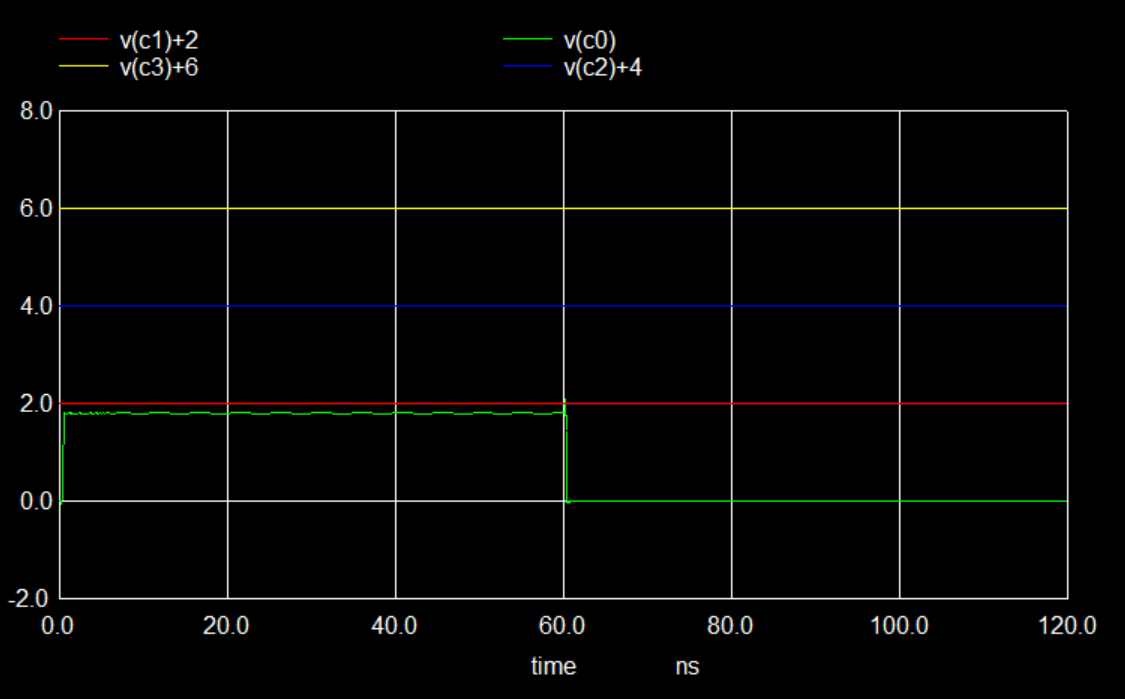
\includegraphics[scale = 0.5]{4_bit_AND_11.png}}
    \caption{ANDing}
    \label{fig:fig21}
\end{figure} \newline 

\subsection{Observation based on Images}
After looking at all the images, we conclude that the MAGIC images are more accurate to suite to the real scenario than
those by any other platform. The occasional \textit{spikes} in MAGIC plots are due to flow of \textbf{back-current} or 
\textbf{leakage-current}. In out design, the spikes seem more prominent due to the non-uniformity across gates, especially
their sizes which differ from gate to gate. Also, the length of the path taken by inputs as well as each intermediate output
to reach the desired destination matters quite significantly when talking about \textit{spikes}.\newline 
Another observation that comes to notice is that if we reduce the amount of time for the pulse, then the \textit{spikes}
become more pronounced in terms of visibility. The reason for this will be cleared in the following section. 

\subsection{Delay Analysis}
One of the most important aspects of Digital IC design is delay analyis. This is a crucial part of the process because 
as a manufacturer you wouldn't want the user to have a bad experience by waiting for the outputs after giving the inputs.
We want the input-to-output response as quick as possible. This also plays an important role in the power consumption of 
the blocks used. \newline 
One of the ways to reduce delays is by increasing the \textbf{Supply}, but that increases the power by a good amount because 
power is quadratically proportional to \textbf{Supply}. \hyperlink{del_tab}{Table 2} shows the comprehensive delay analysis
for each block culminating into a \textbf{4-bit-ALU}, the maximum delay of which will be decided by the block with maximum 
latency. \newline 
Now, as per \hyperlink{del_tab}{Table 2}, we see that the Adder-Subtractor has the highest delay for both inputs and that does make
sense because of the fact that the Full-Adder is being cascaded multiple times. The delay is also maximised due to the path taken by
the inputs which varies for each one, and to add to it, the non-uniformity in the construction of gates (size of transistors)
also plays a big role. Finally, since I have added an enabler-like block at the output-end, a little delay is added by that as
well.
\begin{table}[htp!]
\begin{center} 
\hypertarget{del_tab}{
\begin{tabular}{|p{1.8cm}|p{1.8cm}|p{1.5cm}|p{1.5cm}|p{3cm}|}
    \hline 
    \textbf{Block} & \textbf{Input Combo} & \textbf{input A} (Max delay due to any of its bits) & \textbf{input B} (Max delay due to any of its bits) & \textbf{Explanantion} \\
    \hline
    Adder-Subtractor & A=15, B=0 and A=0, B=15 & 2.54353e-9s & 3.74776e-9s & Delay for B is more because it passes through 
    XOR gates which adds the time.\\
    \hline 
    Comparator & A=15, B=0 and A=0, B=15 and A=15, B=15 & 1.41977e-9s for Gt, 1.53620e-9s for Eq &  1.41114e-9s for Lt, 
    1.52226e-9s for Eq & The delays here for A and B are almost equal due to the symmetry in the circuit\\
    \hline 
    ANDer & A=15, B=15 & 3.41690e-10s & 3.33547e-10s & Delays for A and B are almost equal due to symmetry in the circuit and 
    more interestingly it has the least delay of all blocks due to involvement of only 1 type of gate and without any cascading. \\
    \hline
\end{tabular}}
\caption{Delay Analysis for each block}
\label{tab:t2}
\end{center}
\end{table} \newline
From the \hyperlink{del_tab}{Table 2}, we conclude that the maximum delay for the entire ALU is found in the \textbf{Adder-Subtractor}
block. This delay traces its path from input $B_0$ to $S_3$, passing through an XOR gate to start with and propagating via \textit{carries}
to each cascaded full-adder. It therefore forms the critical path of the \textbf{ALU}. Thus, we can conveniently conclude that the maximum 
delay of the \textbf{ALU} is \textbf{3.74776e-9s}.

\section{Appendix-1 Boolean Logic}
\label{sec:Appendix}
This section deals with the boolean logic used for constructing each block. 
\begin{itemize}
    \item \textbf{Decoder} - This is a simple design that helps the user choose which function to perform based on the select lines.
    The logic for it goes as follows:
    \begin{center}
        $y_0 = Sel_0^cSel_1^c$\\
        $y_1 = Sel_0^cSel_1$\\
        $y_2 = Sel_0Sel_1^c$\\
        $y_3 = Sel_0Sel_1$
    \end{center}
    Where $Sel_0$ and $Sel_1$ are the select lines.
    \item \textbf{Addition} - Here, just the logic for Full-Adder is shown. To make the 4-bit Adder we simply cascade the 
    Full-Adders. The logic goes as follows:
    \begin{center}
        $C_{out} = C_{in}(A\otimes B) + AB$ \\
        $S = C_{in}\otimes (A\otimes B)$
    \end{center}
    where $C_{out}$ is the output carry and $C_{in}$ is the input carry. $S$ is the output sum.\newline 
    Now when we cascade four of these to make a 4-bit Adder, the input carry to the first block is given by the user, but 
    the from the second block onwards, input carry to the block is the output carry of the previous block. The logic goes
    as follows:
    \begin{center}
        $C_{out0} = C_{0}(A_0\otimes B_0) + A_0B_0$ \\
        $S_0 = C_{0}\otimes (A_0\otimes B_0)$

        $C_{out1} = C_{out0}(A_1\otimes B_1) + A_1B_1$ \\
        $S_1 = C_{out0}\otimes (A_1\otimes B_1)$

        $C_{out2} = C_{out1}(A_2\otimes B_2) + A_2B_2$ \\
        $S_2 = C_{out1}\otimes (A_2\otimes B_2)$

        $C_{out3} = C_{out2}(A_3\otimes B_3) + A_3B_3$ \\
        $S_3 = C_{out2}\otimes (A_3\otimes B_3)$
    \end{center}
    $C_{out3}$ becomes the overflow bit for a four-bit adder.
    \item \textbf{Subtraction} - Subtraction is not different that addition if we see the subtrahend as the 2's complement 
    of the number to be subtracted. To get that, we just add a few more gates - XOR gates and pass the bits of B through them.
    \begin{center}
        $B_{eff0} = B_0\otimes C_0$\\
        $B_{eff1} = B_1\otimes C_0$\\
        $B_{eff2} = B_2\otimes C_0$\\
        $B_{eff3} = B_3\otimes C_0$
    \end{center}
    Finally, in the previous logic for the Full-Adders (in the cascaded ones as well) we simply replace $B_i$ with $B_{effi}$. 
    These gates together with the cascade form the 4-bit Adder.
    \item \textbf{Comparator} - Given two 4-bit numbers, we basically need to output whether $A>B$ or $A<B$ or $A=B$. The 
    boolean logic for the same goes as follows:
    \begin{center}
        $Eq = (A_0\otimes B_0)^c(A_1\otimes B_1)^c(A_2\otimes B_2)^c(A_3\otimes B_3)^c$
    \end{center} 
    Now let $x_i = (A_i\otimes B_i)^c$, then 
    \begin{center}
        $Gt = (A_3B_3^c) + x_3(A_2B_2^c) + x_3x_2(A_1B_1^c) + x_3x_2x_1(A_0B_0^c)$
        $Lt = (A_3^cB_3) + x_3(A_2^cB_2) + x_3x_2(A_1^cB_1) + x_3x_2x_1(A_0^cB_0)$
    \end{center}
    where $Eq$, $Gt$ and $Lt$ represent $A=B$, $A>B$ and $A<B$ respectively.
    \item \textbf{ANDer} - This is a very straightforward block whose logic is as follows:
    \begin{center}
        $C_0 = A_0B_0$\\
        $C_1 = A_1B_1$\\
        $C_2 = A_2B_2$\\
        $C_3 = A_3B_3$
    \end{center}
    where, $C_0$, $C_1$, $C_2$ and $C_3$ are outputs.
\end{itemize}
Finally, we combine all of this to make the \textbf{4-bit ALU}, which looks as follows:
\begin{figure}[htp!]
    \centering
    \hypertarget{4ALU}{\rotatebox{90}{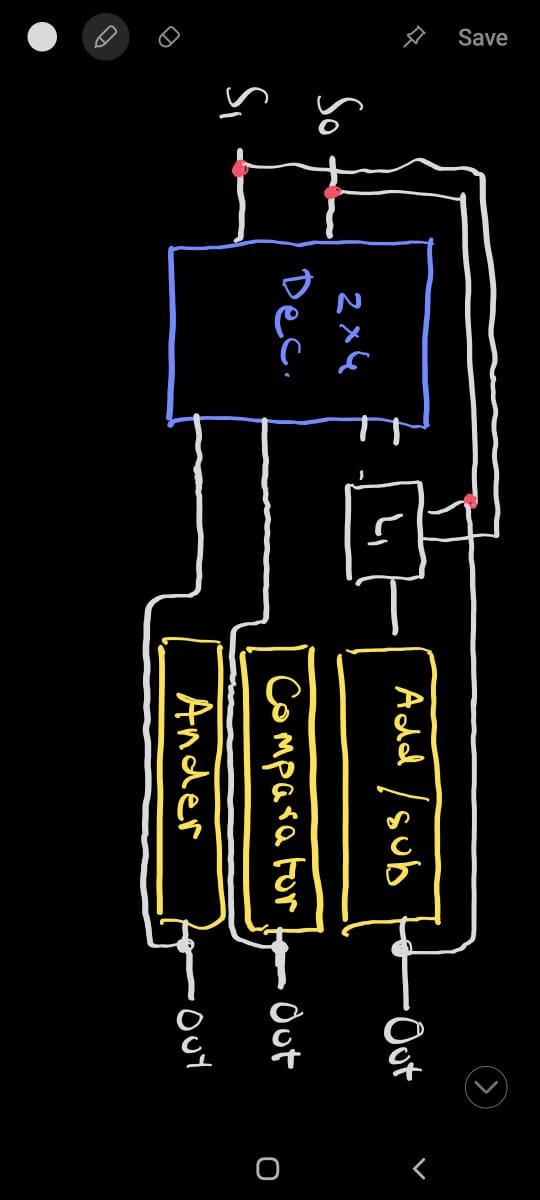
\includegraphics[scale = 0.25]{Image_4-bit_ALU.jpg}}}
    \caption{4-bit ALU}
    \label{fig:fig22}
\end{figure}

\section{Conclusion}
Wo observed that the 4-bit ALU, although very basic as compared to the used ones, served in effectively imparting the 
knowledge that goes into designing and analysing it. It involves usage of multiple blocks which in turn are a combined 
effort of smaller blocks - gates. After designing the logic and coding it in Verilog, we made use of NGSpice to
create the transistor-level netlist. That lead us to its layout design using MAGIC which was again converted back to SPICE
for verification. Finally, we ended the inference wuth delay analysis that was performed to identify the critical path of
the entire circuit starting from the two 4-bit number inputs.
\end{document}